\section{Metode}

Der søges at udregne varmestrømmene for de forskellige komponenter, således at disse kan indgå i sammenligning af varme og temperatur.

\begin{enumerate}
	\item Klarlægning af flowgeometrien
	\item Beregn Referencetemperatur
	\item Bestem kendetal(Re, Gr, Ra, Pr)
	\item Vælg modelligning
	\item Beregn varmeovergangstallet ud fra Nusselts tal
\end{enumerate}

Det antages at processoren afgiver 100 \% af sin varme i kølesystemet.
Systemgrænserne udgøres (som tidligere nævnt) af interfacet til processoren og af bortledning af varme fra den sidste komponent i kølesystemet.
%Vi vil søge at sammenligne den effekt de respektive komponenter bortleder for at kunne sætte et udtryk op for hvor meget strøm Processoren kan afsætte.

FIXME: Her bør være en illustration set fra siden.
\begin{figure}
	\centering
	\includegraphics[width=0.7\linewidth]{"../../../../../../../one drive/OneDrive - Aarhus universitet/TD projekt/KF.png}
	\caption{kontrolflader for systemet der regnes på.}
	\label{fig:kf}
\end{figure}

\begin{figure}
	\centering
	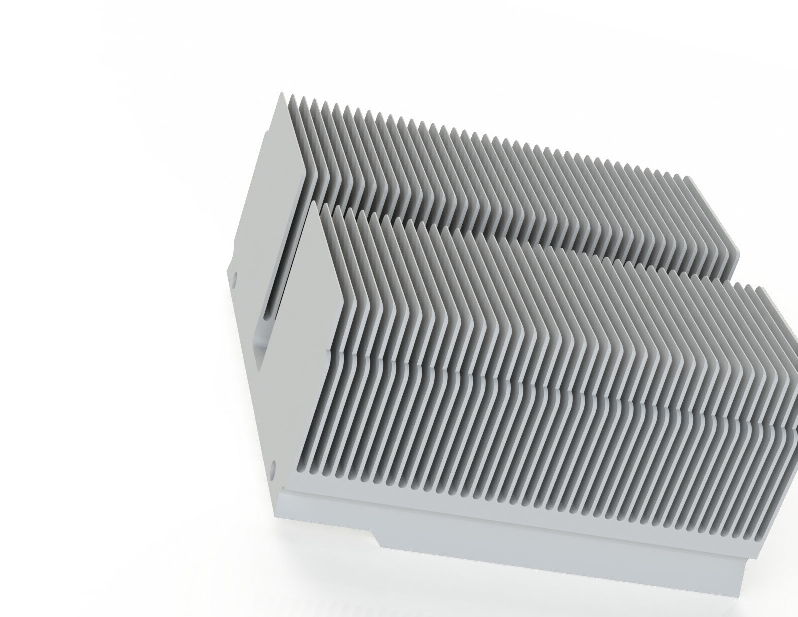
\includegraphics[width=0.7\linewidth]{billeder/heatsink1}
	\caption{Eksempel på kølegitter, fra grabcad.com - bruger: Fernando}
	\label{fig:heatsink1}
\end{figure}


\begin{figure}
	\centering
	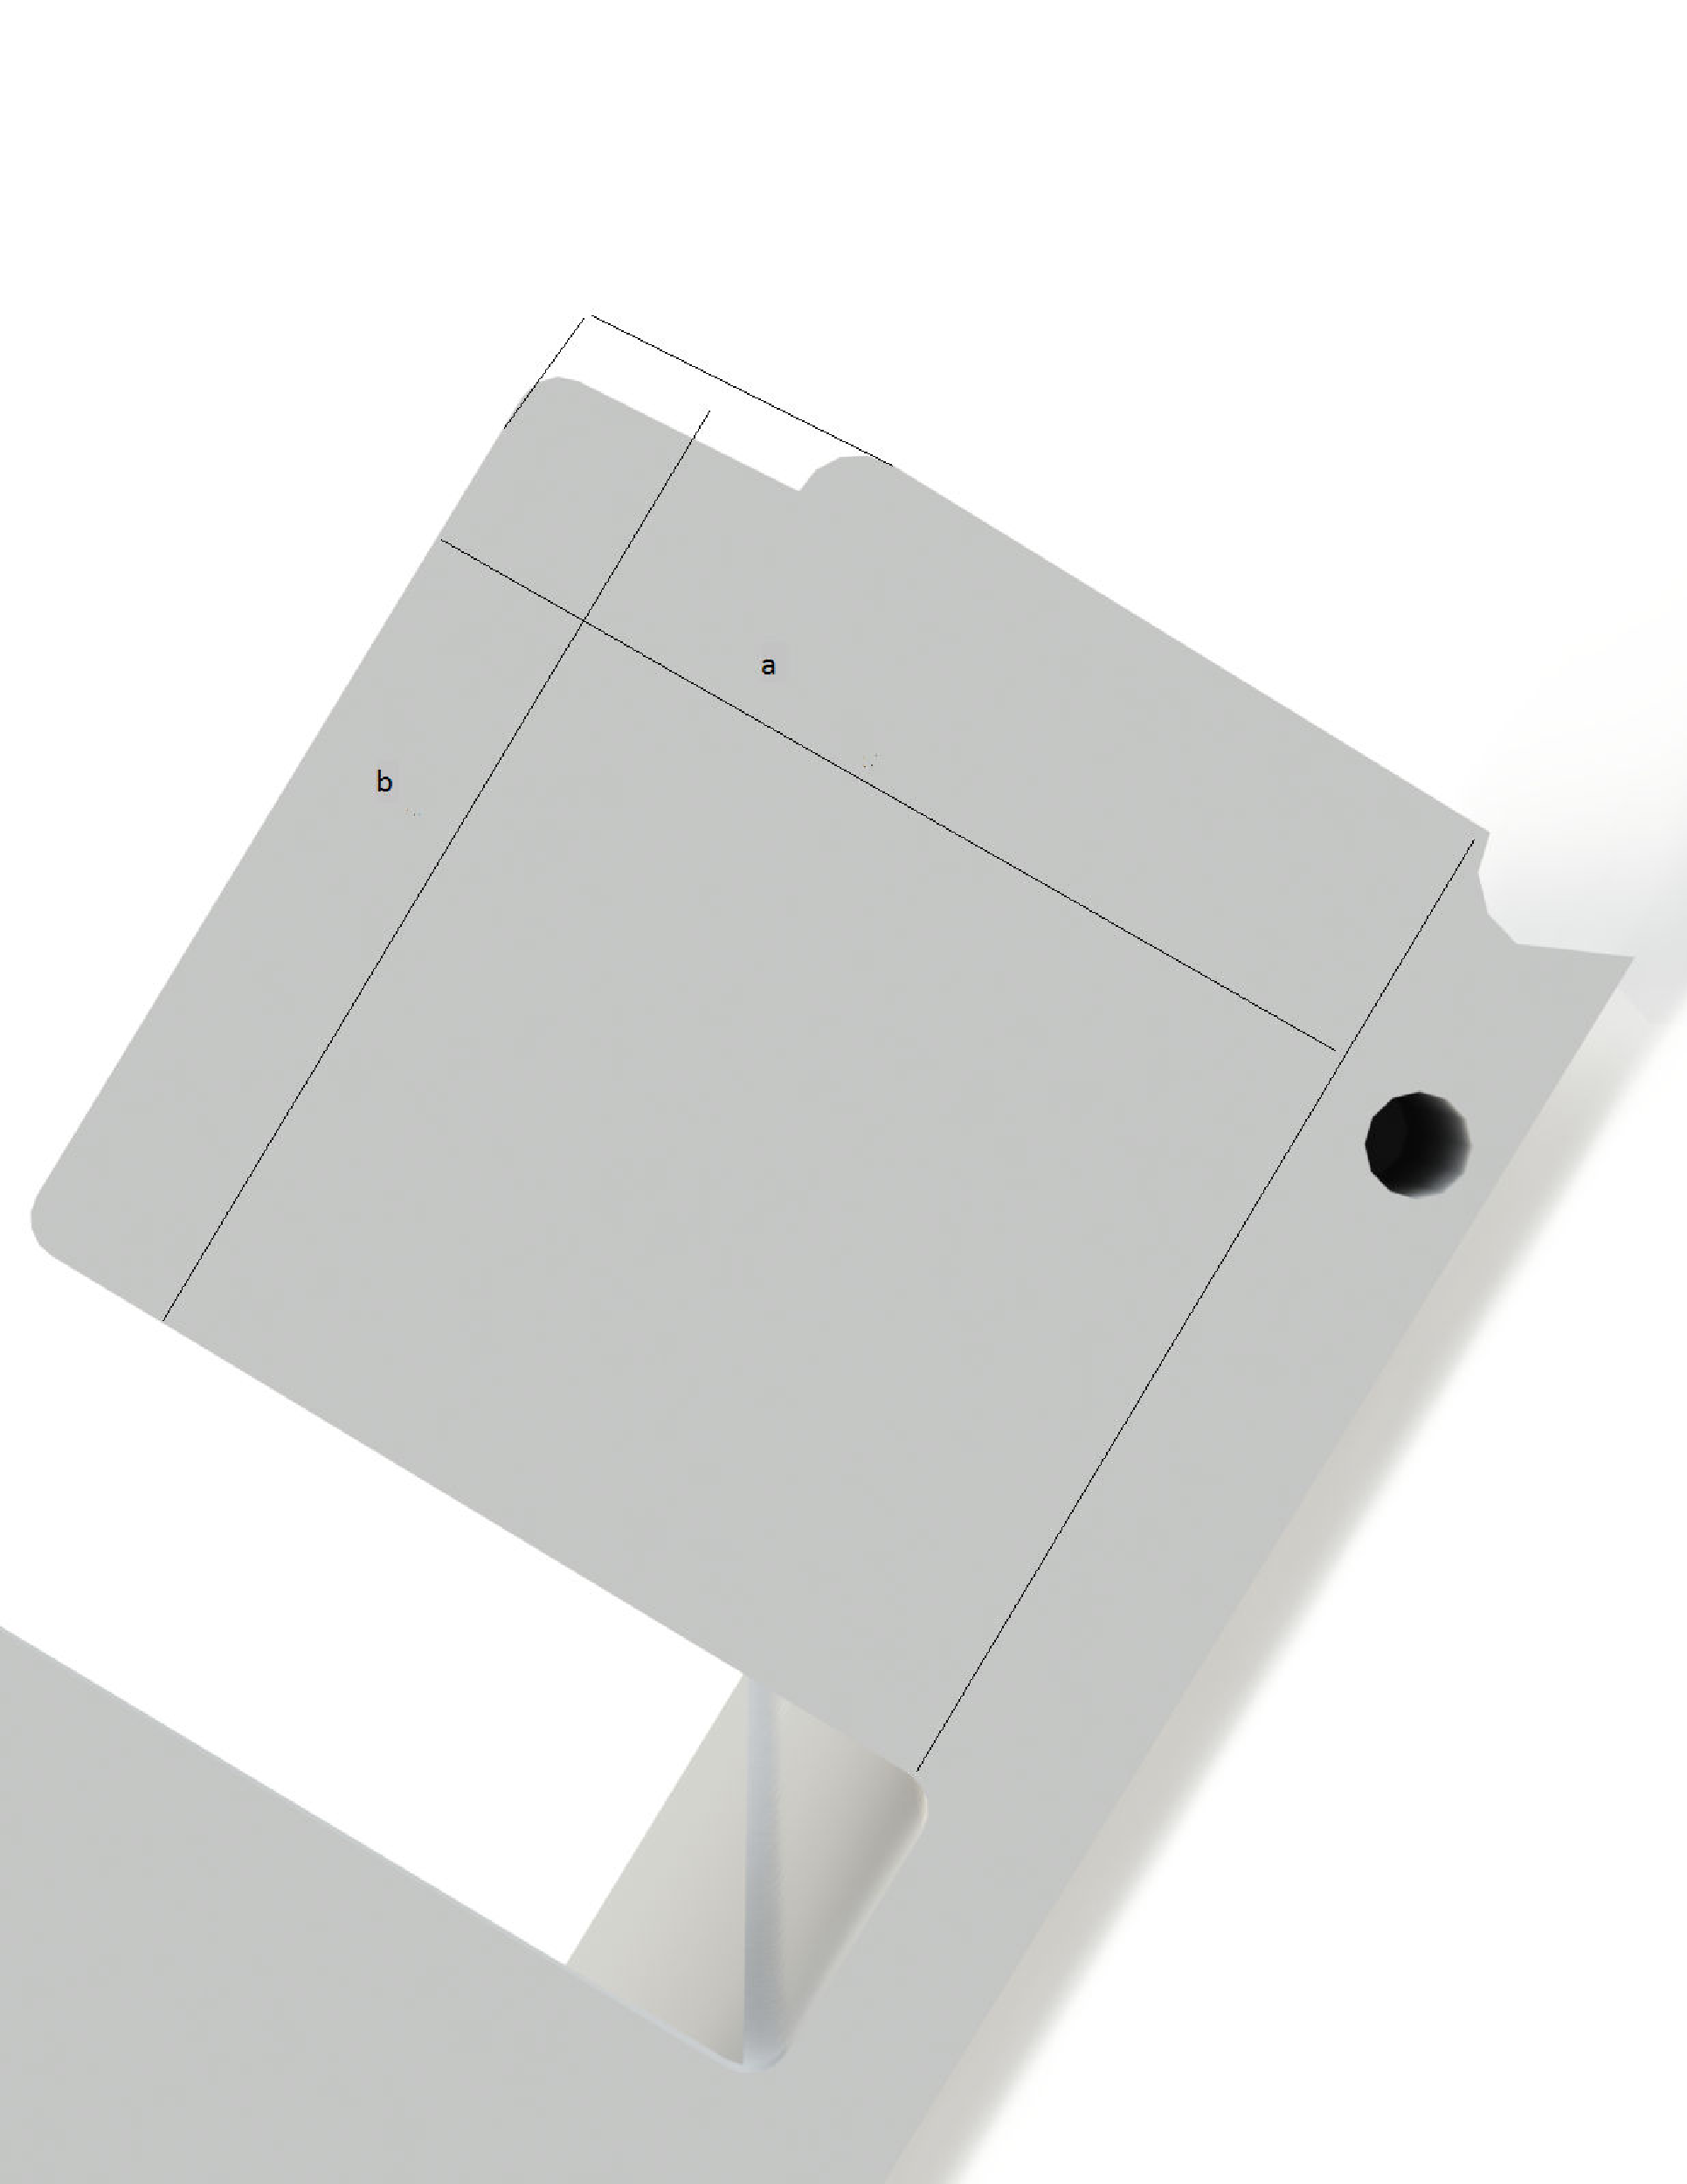
\includegraphics[width=0.7\linewidth]{billeder/lamel}
	\caption{Lamel. Genstand for vore termdynamiske undersøgelser. fra grabcad.com - bruger: Fernando}
	\label{fig:lamel}
\end{figure}